\documentclass[11pt,a4paper,hidelinks]{article}
\bibliographystyle{ieeetr}
\usepackage{setspace}
\doublespacing
\usepackage{graphicx}
\usepackage{biblatex} 
\addbibresource{literature.bib}
\usepackage{ragged2e}
\usepackage{geometry}
\usepackage{marvosym}
\usepackage{wrapfig}
\usepackage{subfig}
\usepackage{textcomp}
\usepackage{hyperref}
\usepackage{rotating}
\usepackage{pdfpages}
 \geometry{
 a4paper,
 %total={170mm,257mm},
 left=20mm,
 right=20mm,
 top=20mm,
 bottom=20mm,
 } 
 \usepackage{fontspec}
\setmainfont{Calibri}
%%https://tex.stackexchange.com/questions/44618/dynamically-count-and-return-number-of-words-in-a-section
%%Taken from Stack Exchange. Steven B. Segletes
\usepackage{tokcycle}[2021-03-10]
\usepackage{xcolor}
\newcounter{wordcount}
\newcounter{lettercount}
\newcounter{wordlimit}
\newif\ifinword
% USER PARAMETERS
\newif\ifrunningcount
\newif\ifsummarycount
\def\limitcolor{red}
\setcounter{wordlimit}{0}
%%
\makeatletter
% \tc@defx is like \def, but expands the replacement text once prior to assignment
\newcommand\addtomacro[2]{\tc@defx#1{#1#2}}
\newcommand\changecolor[1]{\tctestifx{.#1}{}{\addcytoks{\color{#1}{}}%
  \tc@defx\currentcolor{#1}}}
\makeatother
\newcommand\dumpword{%
  \addcytoks[1]{\accumword}%
  \ifinword\stepcounter{wordcount}
    \ifrunningcount\addcytoks[x]{$^{\thewordcount,\thelettercount}$}\fi
    \ifnum\thewordcount=\value{wordlimit}\relax\changecolor{\limitcolor}\fi
  \fi%
  \inwordfalse
  \def\accumword{}}
\newcommand\addletter[1]{%
  \tctestifcatnx A#1{\stepcounter{lettercount}\inwordtrue}{\dumpword}%
  \addtomacro\accumword{#1}}
\xtokcycleenvironment\countem
  {\addletter{##1}}
  {\dumpword\groupedcytoks{\processtoks{##1}\dumpword\expandafter}\expandafter
    \changecolor\expandafter{\currentcolor}}
  {\dumpword\addcytoks{##1}}
  {\dumpword\addcytoks{##1}}
  {\stripgroupingtrue\def\accumword{}\def\currentcolor{.}
    \setcounter{wordcount}{0}\setcounter{lettercount}{0}}
  {\dumpword\ifsummarycount\tcafterenv{%
    \par(Wordcount=\thewordcount, Lettercount=\thelettercount)}\fi}
\begin{document}
\pagenumbering{gobble}
\begin{titlepage}
	\centering
	{Imperial College London - Cancer \& Surgery}\\
	\vspace{12cm}
	{\huge{SPIB - A potential biomarker in breast cancer?}}\\
	\vspace{3cm}
	Jan-Philipp Cieslik (CID 02139878) \\
	\vspace{3cm}
	The R code is included in the appendix. \\
	The R-Markdown notebook and the \LaTeX source files are published on GitHub. \url{https://github.com/jan-cieslik/mres_assignment}\\
	\vspace{1cm}
	Word Count: 1277
    
\end{titlepage}

\newpage
\justifying
\pagenumbering{arabic} 

%\summarycounttrue

% !TEX root = ../main.tex
\section{Introduction}
\countem

Breast cancer is the\ most common cancer in women.
One in every seven women in the UK will be diagnosed with breast cancer in their lifetime. 
Due to the high incidence, breast cancer is also accountable for the most cancer\-/associated deaths.
To predict patient outcomes and to find new actionable targets for cancer therapy new biomarkers are required.
There is already a multitude of established clinical markers like the tumour size, lymphatic node invasion status, distant metastasis status (as in the TNM classification) and molecular characterization (mainly oestrogen, progesterone and HER2 receptor status).
High throughput data is becoming more readily available, allowing for in silico analysis of multiomics (e.g., genomics, proteomics, \ldots) of large cohorts.
This essay tries to demonstrate the utility of Spi-B as a possible breast cancer biomarker.
The transcription factor Spi-B is encoded by the gene SPIB and is a member of the Erythroblast Transformation Specific (ETS) group, which is defined by a common highly conserved DNA\-/binding domain.
In the literature Spi-B is described as both a tumor suppresor and an oncogenic protein.
Studies in lung cancer cells found Spi-B to be involved in recruitment of tumor associate macrophages (TAM) \cite{Huang2021}, further Spi-B was found to promotes anoikis resistance \cite{Zhang2020}.
\endcountem \\
(Introduction word count: \thewordcount{)

% !TEX root = ../main.tex
\section{Methods}
\countem

\subsection{Data Sources}

The Cancer Genome Atlas (TCGA) dataset for breast cancer (BRCA)\cite{Ciriello2015} was acquired from the Xena platform \cite{Goldman2018}.

\subsection{Data Pre-Processing and Normalization}

Some data was downloaded after pre-processing steps have already been performed.
I will outline all important data pre-processing steps to give a complete representation of the resulting data.

\subsubsection{RNA-Seq}

Gene expression profiles from the Illumina HiSeq 2000 RNA sequencing platform were aligned and annotated using reference transcripts based on the hg19 reference genome.
Transcript abundance was calculated with RSEM (RNA-Seq by Expectation Maximization) and transformed to log2(x+1) normalized values.

\subsubsection{Methylation}

Methylation data from the Illumina Infinium HumanMethylation450 BeadChip (Methylation450k) was transformed into $\beta$ values ranging from 0 to 1.
A higher $\beta$ value indicates a higher level of DNA methylation.
The probes were aligned to the hg19 reference genome.
Methylation probes were then annotated with their corresponding gene symbol.

\subsubsection{Copy Number}

Copy number data was obtained via a whole genome microarray.
The raw data was processing using the GISTIC2 (Genomic Identification of Significant Targets in Cancer) pipeline.
Finally, the resulting values were grouped by thresholds and transformed into one of five levels from deep deletion (-2) to high-level amplification (+2).

\subsection{Identification of a Possible Novel Prognostic Marker}

A multivariate Cox proportional hazards regression model was created with data from 1218 breast cancer patients.
Overall survival was defined as the dependent (outcome) variable while mRNA log values (as determined by RNA sequencing from the primary tumour) together with age and tumour stage (I/II as low; III/IV as high) were defined as the independent variables.
The calculated p-values were corrected with the false discovery rate (FDR) method and are shown as q-values.

\subsection{Survival Analysis}

The patient population was divided into SPIB-high and SPIB-low based on the median of the SPIB mRNA expression.
A logrank test and an associated Kaplan-Meier plot were generated for the two subpopulations.

\subsection{Methylation and mRNA Expression Correlation}

Methylation values were tested for normal distribution using Shapiro-Wilk normality test.
The $\beta$ values fail to show a normal distribution (e.g., cg07979271: ${p < 2.2 \cdot 10^{-16}}$), consequently a nonparametric test was used for correlation.
Methylation $\beta$ values were correlated against the mRNA log values using spearman.
P-values were corrected for multiple testing by using FDR and transformed into q-values.
The most anti-correlated methylation site is then shown as a scatter plot against the mRNA level.

\subsection{Copy Number and mRNA Expression}

A chart with multiple box plots (one per copy number threshold) was generated displaying the corresponding mRNA log values.
To test for dependence of mRNA expression on copy number I performed a one-way independent ANOVA (analysis of variance).

\subsection{mRNA Co-Expression}

mRNA expression values were correlated with the corresponding expression values of SPIB using spearman.
The p-values were adjusted for multiple testing by using FDR and transformed into q-values.
\\
\endcountem
(Methods word count: \thewordcount{})

% !TEX root = ../main.tex
\section{Results}
\countem
\subsection{Identification of a possible novel prognostic marker}
In a multivariate Cox analysis in 1218 breast cancer patients I could identify 2078 significantly (q-value < 0.05) associated genes with the overall survival.
SPIB was associated with a beneficial harzard ratio (HR: 0.91; q-value: 2.82\%).
\endcountem \\
(Results word count: \thewordcount{})

% !TEX root = ../main.tex
\section{Conclusion}
\countem
...
\endcountem \\
(Conclusion word count: \thewordcount{})

\newpage
% !TEX root = ../main.tex
\section{Figures and Tables}

\begin{figure}[h!]
    \centering
    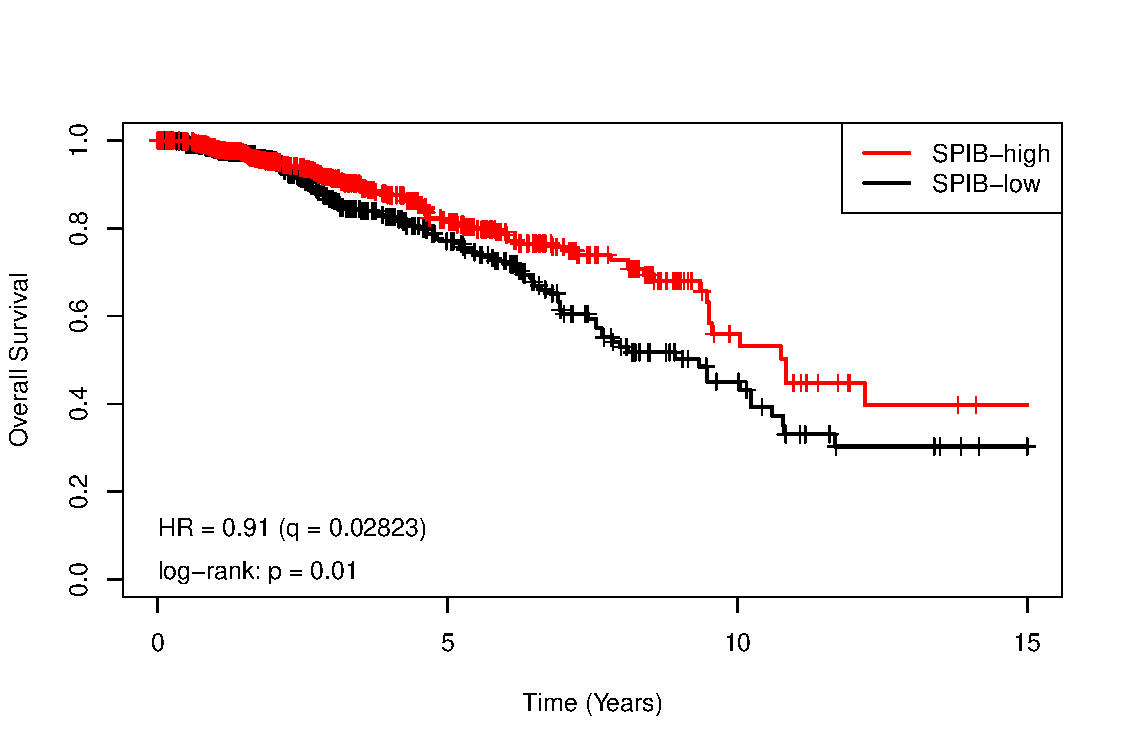
\includegraphics[scale=0.75]{figures/km_plot.pdf}
    \caption{Survival of SPIB-high and SPIB-low breast cancer patients. Data from the TCGA dataset \cite{Ciriello2015, Goldman2018}}
    \label{km_plot}
\end{figure} 

\begin{figure}[h!]
    \centering
    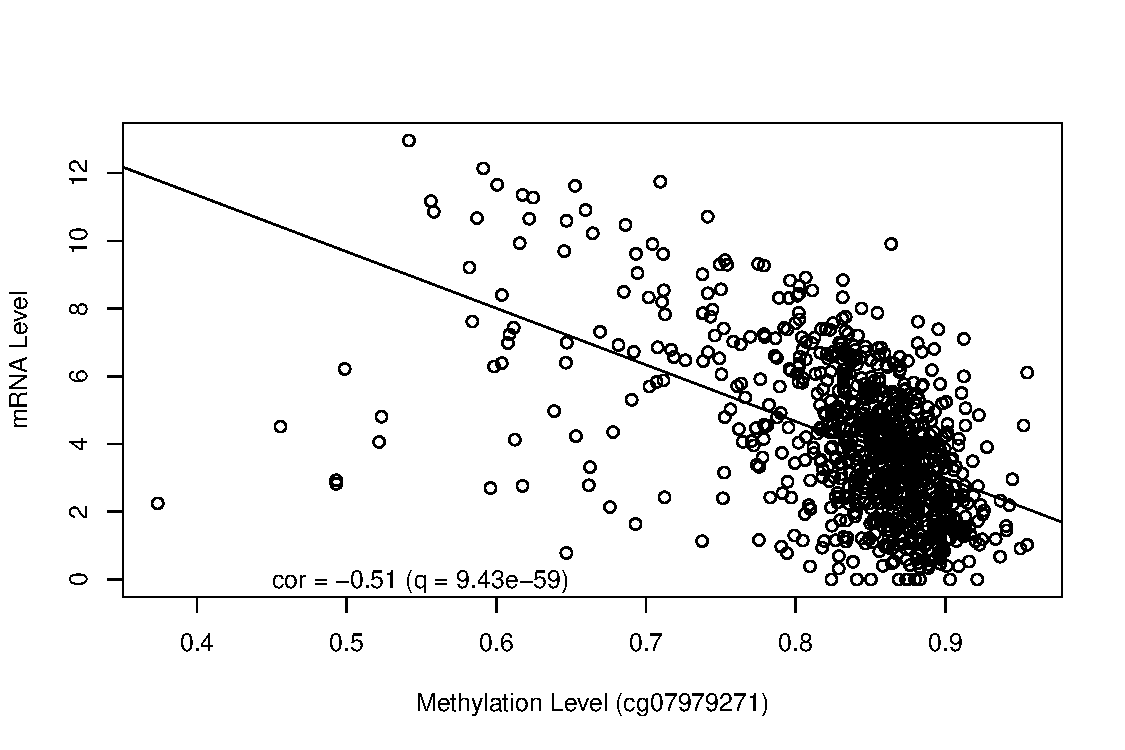
\includegraphics[scale=0.75]{figures/methylation.pdf}
    \caption{methylation \cite{Ciriello2015, Goldman2018}}
    \label{methylation}
\end{figure} 

\begin{figure}[h!]
    \centering
    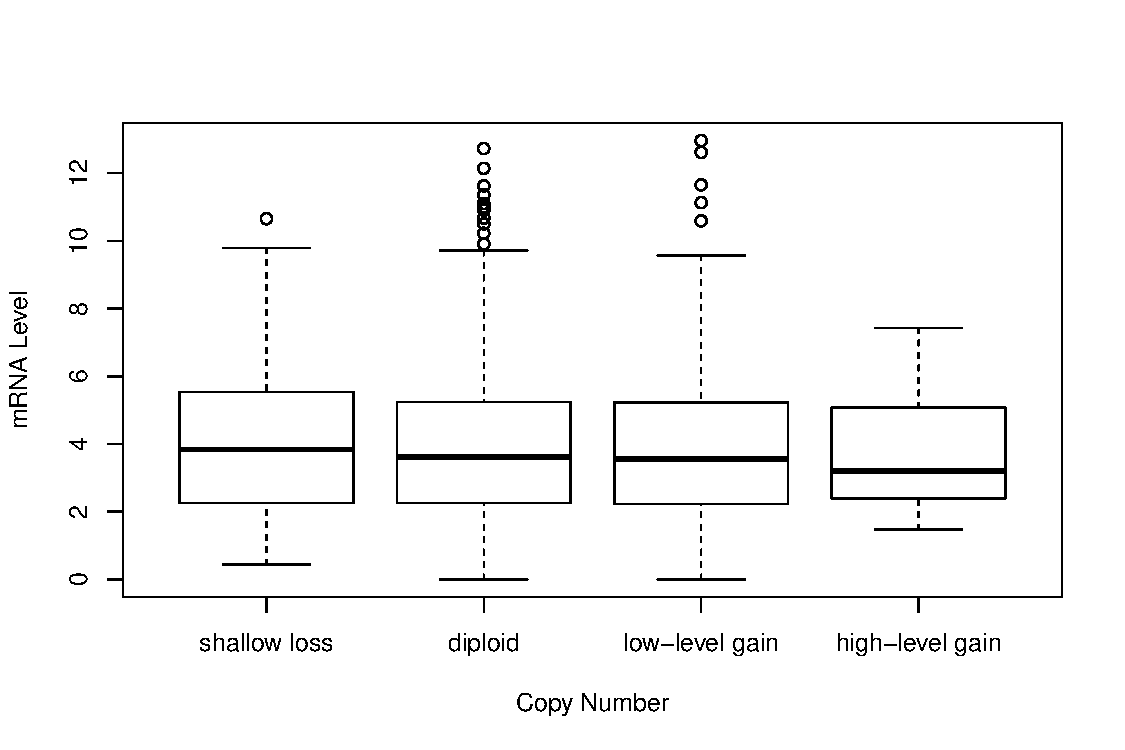
\includegraphics[scale=0.75]{figures/cnv.pdf}
    \caption{Copy number alteration \cite{Ciriello2015, Goldman2018}}
    \label{cnv}
\end{figure} 
 
\newpage
\printbibliography

\newpage
\pagenumbering{gobble} 

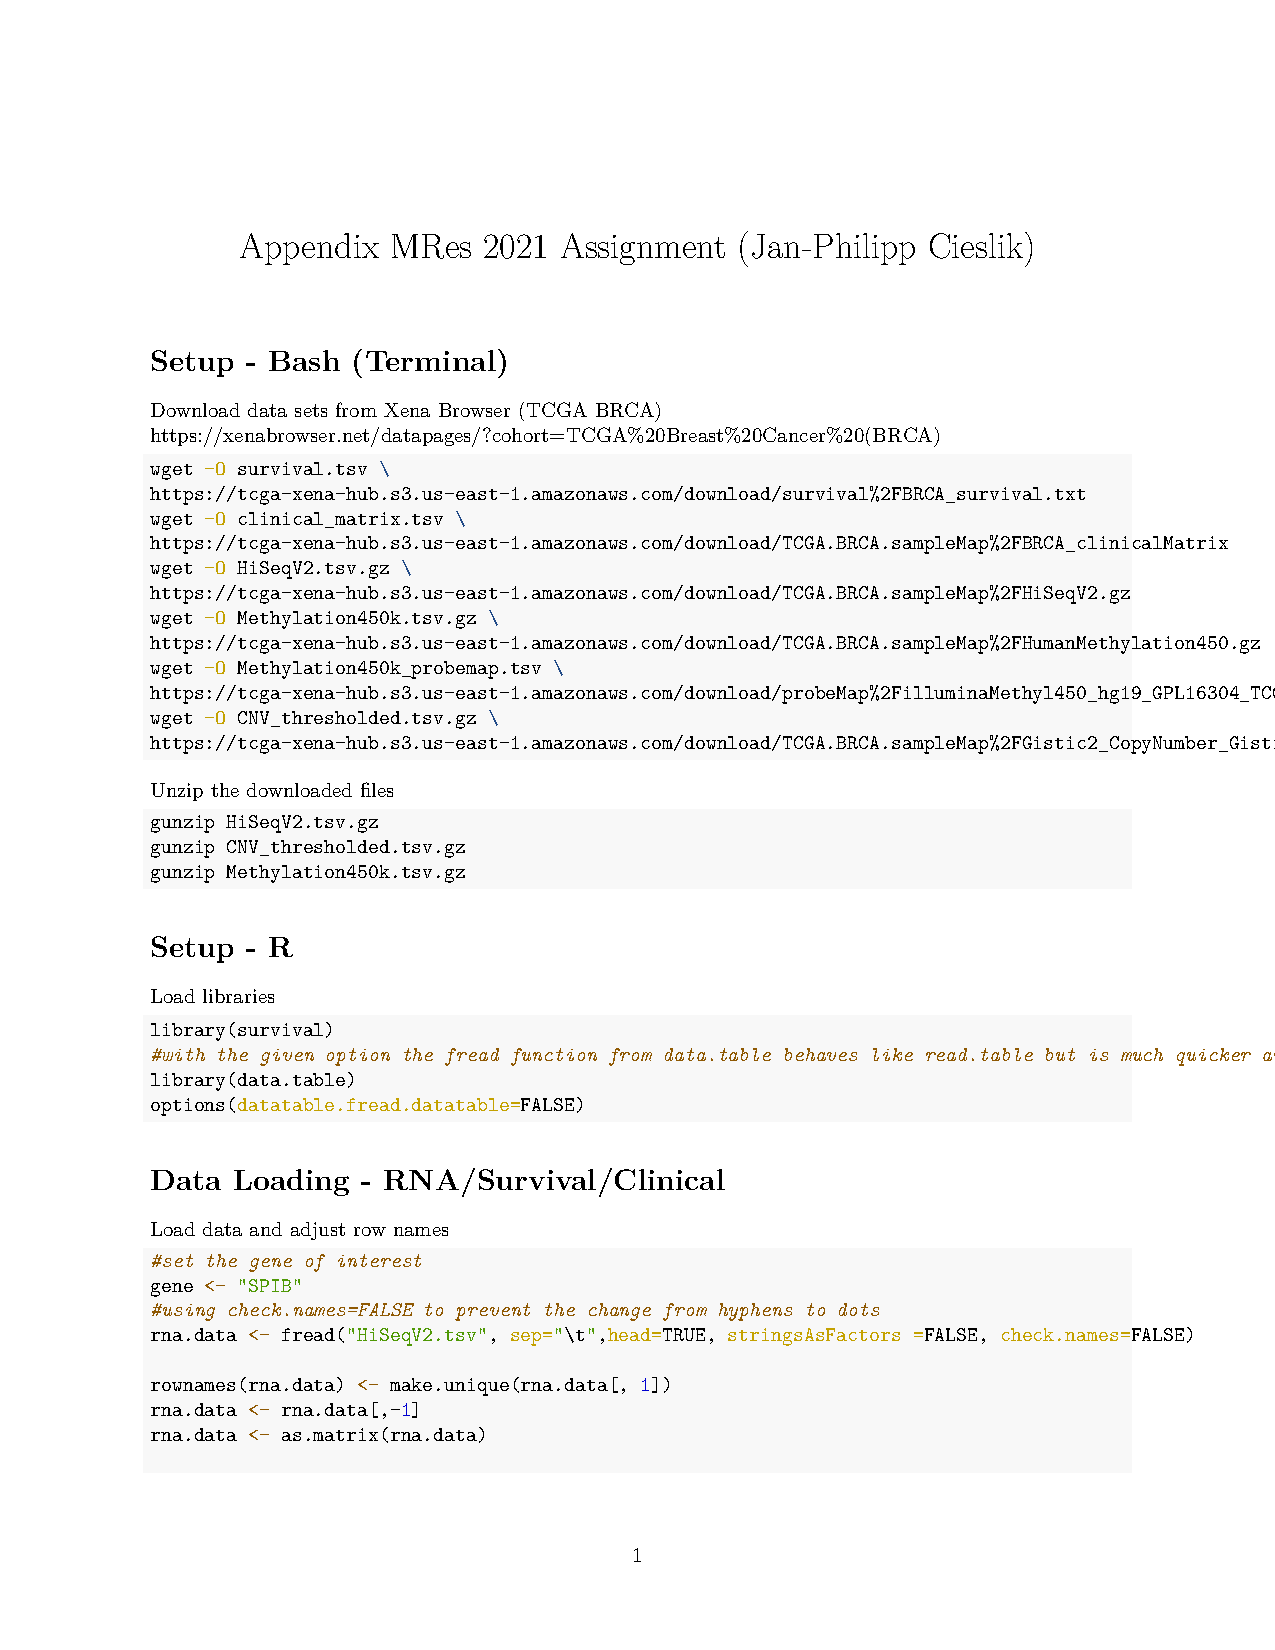
\includepdf[pages=-]{../data/assignment.pdf}

\end{document}